\documentclass[letterpaper,12pt]{scrartcl}
\usepackage[utf8]{inputenc}
\usepackage{amsmath}
\usepackage{amssymb}
\usepackage{graphicx}

\title{Amateur Radio Basic Qualification -- The Essentials}
\subtitle{Sections Four and Five: Electronic Devices}
\author{University of Waterloo Amateur Radio Club}
\date{\today}

\begin{document}

\maketitle
\tableofcontents

\section{Introduction}

%These notes were prepared from Issue 3 of RIC-7 ``Basic Qualification Question Bank for Amateur Radio Operator Certificate Examinations'', published April 2007.
%They cover 100\% of testable material on the Basic Qualification examination, but do not go beyond what is absolutely necessary to know in order to pass the examination.
%The candidate is encouraged to perform their own research on topics that are not fully covered here.

Up until now, these notes have been written with only the most important information in mind and have not covered
a great deal of information that will not be directly tested on the Basic Qualification exam.
When covering the topics of electronic circuits and components, most of the information here will not make sense
without a good background. The goal of this section is to provide that background -- which is not technically covered in the exam,
but should prove extremely useful both for understanding the ideas here and for practical operation --
and to introduce the most important electronic devices in amateur radio one at a time
-- which are pulled from the testable material -- without breaching into the more complex territory of circuit analysis and design.

Also, section five is presented first because it covers the material in the correct order.

\section{The Essentials: Section Five (Passive Devices)}

\subsection{Particle Physics}

\begin{itemize}
\item All matter is made up of atoms, which have a \textbf{nucleus} composed of neutrons (electrically neutral)
and protons (electrically positive) and an \textbf{electron cloud} composed of electrons (electrically negative).
\item In an atom, there are an equal number of protons and electrons. The atom is electrically neutral.
\item An atom can gain electrons, resulting in a \textbf{negative ion}, or lose electrons, resulting in a \textbf{positive ion}.
\item \textbf{Current} is the flow of electric charge (typically the flow of electrons).
\item The unit of electric charge is the coulomb (C). One coulomb is equal to the charge on $6.28 \times 10^{18}$ electrons.
\item Current is measured in coulombs per second, or amperes (A). One ampere equals a flow of one coulomb per second through a conductor
(such as a piece of copper wire).
\item The symbol $I$ is used to denote current in equations. You may also see a lowercase $i$ to indicate a current that changes with time.
\item One way to visualize current is to think of the flow of water in a canal. Here the water represents the electrons, and the canal is the conductor
through which the current flows. The more water that moves past a point in the canal per unit time, the greater the current in the canal.
\item \textbf{Voltage} is another name for ``electrical potential energy''.
\item Voltage can be a bit tricky to understand. Going back to the water analogy, you might be familiar with the effects of gravity on liquids --
water will flow from surfaces at high elevation down to surfaces at low elevation. Similarly, current flows from points in a circuit
at high voltage towards points in a circuit at low voltage.
\item It is important to distinguish between ``conventional current'' and ``electron current'' here.
Back when electricity was just being discovered, it was believed that the particles that moved in a circuit were positively charged, and therefore would
move from high voltage to low voltage. This is known as ``conventional current'' -- thinking about a hypothetical positively-charged current. 
However, this is now known to be incorrect;
we know that electrons move in a circuit, actually from low voltage to high voltage! Thinking of the current in this way,
as a flow of electrons, is called ``electron current''. In most circuits, ``conventional current'' is used.
\item The unit of electrical potential energy is the volt (V).
\item We never measure electrical potential energy directly. Instead we measure the difference in potential between two points in a circuit.
This potential difference is what is commonly referred to as ``voltage''. For example, the voltage rating of a flashlight battery is 1.5~V.
This means that the difference in potential energy between the terminals of the battery is 1.5 volts.
\item The symbol $V$ is used to denote voltage in equations.
\item Most hams will try to tell you that the symbol for voltage is $E$. This is incorrect, and bad engineering practice.
As a good electrician, follow proper engineering convention and use $V$ for voltage!
\item Unfortunately, there are a handful of questions on the Basic Qualification exam that think that $E$ is the symbol for voltage.
Just play along. You know better.
\item \textbf{Resistance} is the inherent opposition to the flow of electrons of a material.
\item The unit of resistance is the ohm ($\Omega$); the symbol for resistance is $R$.
\item The resistance of a given conductor depends on the following factors:
\begin{itemize}
\item The ``specific resistance'' of the material
\item The length of the conductor (longer conductors have a larger resistance)
\item The diameter or cross-section area of the conductor (larger cross-section means \textit{lower} resistance;
think of a water pipe -- the wider pipe allows a larger amount of water to flow)
\item Temperature -- every material has a ``temperature coefficient'', which affects how the resistance of the conductor changes when
the temperature is raised or lowered. For some materials, the resistance increases at higher temperatures; for others, it will decrease.
\end{itemize}
\item The higher the resistance of a material, the more difficult it is to get current to flow through it when a voltage is applied.
\item But \textit{how} difficult? There is an equation called ``Ohm's Law'' that tells us: $I = \dfrac{V}{R}$.
The current that will flow through a resistor is equal to the voltage difference across the terminals of the resistor
divided by its resistance.
\item One ohm is defined as the resistance of a conductor that will allow a current of one amp to flow through it
when a voltage of one volt is placed across it.
\item The reciprocal of resistance is \textbf{conductance}.
\end{itemize}

\subsection{Units and SI Prefixes}

\begin{itemize}
\item Units such as volts and amperes can be prepended with an ``SI prefix'' to change the scale of the unit.
\item For example, the prefix ``mega-'' means ``one million''. So, ``one megadollar'' is short for ``one million dollars''.
``Two point five megadollars'' is short for $\$2,500,000$.
\item Here is a short list of useful SI prefixes:
\begin{itemize}
\item ``tera'' (T) -- $10^{12}$
\item ``giga'' (G) -- $10^{9}$
\item ``mega'' (M) -- $10^{6}$
\item ``kilo'' (k) -- $10^{3}$
\item ``milli'' (m) -- $10^{-3}$
\item ``micro'' ($\mu$) -- $10^{-6}$
\item ``nano'' (n) -- $10^{-9}$
\item ``pico'' (p) -- $10^{-12}$
\end{itemize}
\item So, for example, one megahertz is equivalent to 1000 kilohertz, for example, or in short form, 1~MHz = 1000~kHz.
Both are equivalent to one million hertz (1000000~Hz).
\end{itemize}

\subsection{Conductors, Resistors, and Insulators}

\begin{itemize}
\item Most metals are good \textbf{conductors} of electricity -- they have relatively low resistance.
\item Some materials such as plastic are \textbf{insulators}, which have relatively high resistance and do not conduct electricity very easily.
\item Copper, silver, and aluminum are very good conductors. Lots of electric circuits use copper wires because copper is inexpensive and conducts electricity easily.
\item Glass, plastic, porcelain, and air are good insulators.
\item Gold is not a very good conductor, but it is typically used to plate the ends of connectors because it does not corrode very easily.
\item An \textbf{open circuit} has infinite resistance, and therefore has no current.
\item A \textbf{short circuit} has zero resistance, and passes too much current.
\item Most resistors are made from carbon film.
\end{itemize}

\subsection{Power}

\begin{itemize}
\item When current flows through a conductor, some of the energy in the electrical current is dissipated as \textbf{heat}.
In some cases, this is desired. For example, a hot element on an electric oven is more or less just a really big resistor that can sink a lot of heat.
However, typically producing heat is not the desired function of a circuit and any heat that is dissipated in a component is considered to be ``lost''.
\item Every resistor has a fixed amount of heat that it can dissipate before it is destroyed by the amount of energy that it is encountering.
This limit is measured in \textbf{watts} ($W$), which is the SI unit for \textbf{power}.
\item Power is defined as energy per unit time; one watt is equivalent to one joule of energy per second.
\item A more useful expression in the context of electric circuits is $P = IV$, where $P$ is power, $I$ is current, and $V$ is voltage.
\item A resistor with a voltage drop of 5 volts across its terminals that is passing 3 amps of current is experiencing a total of $(5)(3) = 15$ watts of power.
The resistor's power rating would have to be higher than 15W in order to be suitable for operation in this circuit.
\item Some resistors are physically very large; this improves their power dissipation and allows them to handle much more power.
\end{itemize}

\subsection{Resistors in Series and in Parallel}

\begin{itemize}
\item It is possible to replace combinations of multiple resistors with a single ``equivalent resistor'' of that value
without changing the behaviour of the circuit.

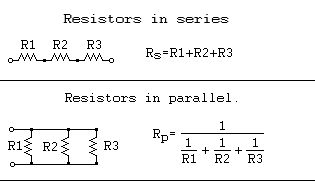
\includegraphics[width=4.0in]{resistors-series-parallel.png}
\item When two resistors are connected with one common terminal, they are said to be connected \textbf{in series}.
\item For any number of resistors connected in series, the total ``equivalent resistance'' is equal to the sum of the resistances of each individual resistor.
\item $R_e = R_1 + R_2 + ... + R_n$
\item For resistors connected in series, the current through each resistor is equal. However, the voltage drop across each resistor
is not necessarily the same.
\item When two resistors are connected with both terminals in common, they are said to be connected \textbf{in parallel}.
\item For any number of resistors connected in parallel, the total ``equivalent resistance'' is equal to one divided by the sum of the reciprocals of the
resistances of each individual resistor.
\item $R_e = \dfrac{1}{\frac{1}{R_1} + \frac{1}{R_2} + ... + \frac{1}{R_n}}$
\item For resistors connected in parallel, the total current through all resistors is equal to the sum of the current through each resistor.
However, the voltage drop across any resistor is the same.
\end{itemize}

\subsection{Resistor Colour Codes}

\begin{itemize}
\item Most resistors are too small for the actual resistance value to be printed on them. Instead, a number of coloured bands are used to indicate
the resistor's value.
\item You will need to memorize the correspondance between band colour and value:

\begin{tabular}{|c|c|}
\hline
Black & 0 \\
Brown & 1 \\
Red & 2 \\
Orange & 3 \\
Yellow & 4 \\
Green & 5 \\
Blue & 6 \\
Violet & 7 \\
Grey & 8 \\
White & 9 \\
\hline
\end{tabular}

\item Most colour-coded resistors have four bands. To calculate the value of a resistor
you only need to know the colours of the first three bands.
Concatenate the digits denoted by the first and second bands, then multiply by 10 to the power of
the third band's digit.
\item As an example, suppose the first three bands of a resistor you have are orange, white, red in that order.
Orange is 3, and white is 9, so the value of the resistor is 39 times some power of 10.
Red is 2, so the value is $39 \times 10^{2}$ or $3900\Omega$.
\item The fourth band represents the tolerance of the resistor's value -- by how much the value of the resistor may vary
from its printed resistance. This is expressed as a percentage value. A 100~Ohm resistor with a tolerance of 5\% will have a \textbf{gold band}
in the fourth position.
\item (Some resistors have five bands. These can be a bit confusing, as there are
two possible ways of reading them: in one case, the first three bands are the first three digits, 
the fourth band is the multiplier, and the fifth band is the tolerance;
in another case, the first four bands are read as on a four-band resistor, and the last band
represents the component failure rate.
There is a very rarely seen six-band resistor. The sixth band represents the temperature coefficient of the device.)
\end{itemize}

% Also covers subsection 6

\subsection{Alternating Current and Electromagnetic Waves}

\begin{itemize}
\item Current that flows in one direction only is called \textbf{direct current (DC)}.
\item Current that oscillates back and forth is called \textbf{alternating current (AC)}.
\item The reversal of the direction of current happens periodically. The number of reversals per second is known as the \textbf{frequency} of the current.
\item In North America, current alternates at a rate of 60 cycles per second, or 60~Hz.
\item Most humans can hear sounds at frequencies between 20 and 20~000~Hz. (But these are sound waves, not electromagnetic waves.
Here the frequency refers to how many times per second the air molecules vibrate in order to propagate the sound wave.)
Signals with these frequencies are known as ``Audio Frequency (AF)'' signals.
\item Signals at frequencies from 3~kHz to 300~GHz are known as ``Radio Frequency (RF)'' signals. \\
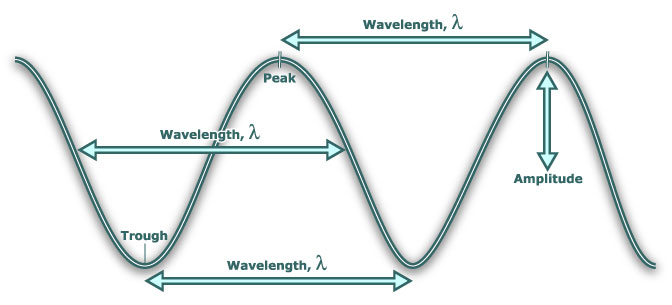
\includegraphics[width=4.0in]{wave.jpg}
\item There is a simple relationship between frequency and wavelength for an electromagnetic wave: $c = \lambda f$, where $\lambda$ is the wavelength
(in meters), $f$ is the frequency (in Hertz), and $c$ is the speed of light ($299792458$ meters per second, or approximately 300 million meters per second).
\item From this you can see that because the speed of light is a constant, as the frequency of a wave increases its wavelength decreases,
and vice versa.
\item The \textbf{period} of a wave is the time required for one complete cycle of the wave to be observed. The period is usually denoted
with the variable $T$, and can be calculated as $T = \dfrac{1}{f}$. So, if the frequency of a wave is 100~Hz,
its period is $\dfrac{1}{100}$, or 0.01 seconds.
\item The \textbf{amplitude} of a wave is the distance between the highest point (the crest) and the lowest point (the trough).
\end{itemize}

\subsection{Decibels}

\begin{itemize}
\item To express the ratio between two values -- mostly power -- we can use the decibel (dB).
\item The ratio of a power value $P_1$ to another power value $P_0$ can be expressed in decibels using the following identity:
$L_{dB} = 10 \log_{10} \dfrac{P_1}{P_0}$
\item From this you can see that a ``10~dB'' increase is an increase of a factor of 10, while a ``20~dB'' increase is an increase
of a factor of 100.
\item Doubling the power corresponds to a gain of roughly 3~dB.
\end{itemize}

\subsection{Capacitors and Inductors}

\begin{itemize}
\item An \textbf{inductor} is an electronic device that can store energy in a magnetic field. Physically it looks like a spiral coil of wire, or a wire wrapped around a ``doughnut'' core (torus).
\item Inductors are sometimes called ``coils''.
\item Inductance is the ability of an inductor to store and supply energy through a magnetic field. The unit of inductance is the henry (H).
\item The symbol for inductance is $L$.
\item The inductance of an inductor depends on the core material, the core diameter, the length of the coil, and the number of turns of wire used to wind the coil.
\item Just like resistors do, inductors that are connected in series or in parallel can be added together.
\item For inductors connected in series, the total equivalent inductance is equal to the sum of each individual inductance.
\item For inductors connected in parallel, the total equivalent inductance is given by $\dfrac{1}{\frac{1}{L_1} + \frac{1}{L_2} + ... + \frac{1}{L_n}}$
(similar to the formula for resistors in parallel).
\item A \textbf{capacitor} is an electronic device that stores energy in an electric field. It is the dual of the inductor. Physically, it looks like a small metal can with two terminals coming out
(although this actually describes a fair number of components), or a small flat circular disk with two terminals coming out.
\item A capacitor is made from two parallel plates separated by some distance. Between the plates there can be a material, known as a \textbf{dielectric}.
\item Capacitance is the ability of a capacitor to store and supply energy through an electric field. The unit of capacitance is the farad (F).
\item The symbol for capacitance is $C$.
\item The capacitance of a capacitor depends on the material between the plates, the area of each plate, the number of plates, and the distance between the plates.
\item Capacitors can also be combined in series or in parallel, but the formulas are the other way around. Capacitors in \textit{parallel} add their capacitances together,
and capacitors in series have a total capacitance equivalent to $\dfrac{1}{\frac{1}{C_1} + \frac{1}{C_2} + ... + \frac{1}{C_n}}$. This is the opposite of how resistors and inductors behave.
\end{itemize}

\subsection{Transformers and also Magnets}

\begin{itemize}
\item Electric current moving through a conductor produces a magnetic field around the conductor. The strength of this magnetic field is directly proportional to the current in the conductor.
\item A voltage can be induced in a conductor when the conductor moves through a magnetic field. This voltage is at a maximum when the movement is perpendicular to the magnetic field lines (``lines of force'').
\item The maximum induced voltage in a coil occurs when the current is going through its greatest rate of change.
\item Two nearby inductors can be ``magnetically coupled'' if they share the same magnetic field.
\item \textbf{Mutual inductance} is the phenomenon whereby a changing current in one inductor causes a current to be induced in another inductor.
\item A \textbf{transformer} is a device that uses mutual inductance to induce a voltage or current in another part of a circuit.
\item A transformer has two coils, known as the ``primary'' and ``secondary''. A flow of current through the primary causes a flow of current through the secondary, by induction.
\item The magnitude of the voltage induced in the secondary depends on the ratio of the number of turns in the primary and secondary. This is given by $\dfrac{V_2}{V_1} = \dfrac{N_2}{N_1}$,
where $V_2$ is the voltage across the secondary, $V_1$ is the voltage across the primary, and $N$ is the number of turns in the corresponding coil.
The quantity $\dfrac{N_2}{N_1}$ is known as the ``turns ratio'' of the transformer (e.g. a transformer with a turns ratio of 5:2 has $\dfrac{N_2}{N_1} = \frac{5}{2}$.
\item The total amount of power transferred through an ideal transformer is constant. That is, $V_1 I_1 = V_2 I_2$. 
(So, a transformer that steps up the voltage must also step down the current.)
\item In a real transformer, energy transfer is not perfect and some power is lost. This might be dissipated as heat, for example.
\item If no load is attached to the secondary winding of a transformer, the current in the primary winding is called ``magnetizing current''.
\item Transformers can be used to match impedances through the formula $\dfrac{Z_2}{Z_1} = \dfrac{N_{2}^2}{N_{1}^2}$
where $N_1$ is the number of turns in the primary, $N_2$ is the number of turns in the secondary, and both $Z$s are given in ohms.
\item A force of repulsion exists between two like magnetic poles (North repels North, South repels South).
\item Good permanent magnets can be made from steel. \textit{Really} good permanent magnets are made from neodymium, or some alloys.
\end{itemize}

\subsection{Reactance}

\begin{itemize}
\item Reactance is defined as the opposition to the flow of alternating current.
\item Reactance is very similar to resistance, and it is also given in ohms. However, the symbol for reactance is $X$.
\item Unlike a resistor, energy dissipated through a reactive component is always returned to the circuit.
\item Reactance is \textbf{frequency-dependent}.
\item The reactance of an inductor is given by $X_L = 2 \pi f L$, where $f$ is the frequency of the alternating current in Hertz
and $L$ is the inductance in Henrys.
\item As the frequency increases, so does the inductive reactance.
\item The reactance of a capacitor is given by $X_C = \dfrac{1}{2 \pi f C}$, where $f$ is the AC frequency in Hertz and $C$ is the capacitance in Farads.
\item As the frequency increases, the capacitive reactance decreases.
\item When a circuit contains both resistance and reactance, it is useful to refer to a combined quantity known as \textbf{impedance}.
\item Impedance is also measured in ohms, but uses the symbol $Z$.
\item \textbf{Impedance matching} refers to the condition when two circuits connected to each other have the same impedance.
Maximum power transfer occurs when the impedances are equal.
\end{itemize}


\subsection{Resonance and Tuned Circuits}

\begin{itemize}
\item Resonance occurs when the inductive reactance, $X_L$, and the capacitive reactance, $X_C$, are equal.
This occurs at exactly one frequency in a circuit, known as the \textbf{resonant frequency}.
\item The formula to calculate the resonant frequency is $f = \dfrac{1}{2 \pi \sqrt{LC}}$, where $f$ is the resonant 
frequency in Hertz, $L$ is the inductance in henries, and $C$ is the capacitance in farads.
\item If we use a component in a circuit whose capacitance or inductance can be adjusted,
we have created a \textbf{tuned circuit}, which can be used to select one frequency from many.
\item A series resonant circuit consists of an inductor and a capacitor connected in series.
\item At resonance, a series resonant circuit has \textit{minimum impedance}. This can be used to select
one frequency from many others.
\item A parallel resonant circuit consists of an inductor and a capacitor connected in parallel.
\item At resonance, a parallel resonant circuit has \textit{maximum impedance}. This can be used to reject a specific frequency
 and pass all others.
\end{itemize}

\subsection{Test Equipment}

\begin{itemize}
\item A \textbf{voltmeter} measures voltage. It has two probes that must be connected in \textit{parallel} with the circuit where the voltage is to be measured.
\item An \textbf{ammeter} measures current. It also has two probes but must be connected in \textit{series} where the current is to be measured.
\item A multimeter, according to Industry Canada, measures voltage, current, and resistance.
\item An ammeter in a circuit will act as a very small resistance. A voltmeter in a circuit will act as a very large resistance.
\end{itemize}

\section{The Essentials: Section Four (Active Devices)}

\subsection{Amplifiers}

\begin{itemize}
\item An amplifier is a circuit designed to increase the level of its input signal.
\item The increase in signal level by an amplifier is called \textbf{gain}, which is usually measured in decibels
(and is a positive number of decibels for an amplifier).
\item Because this adds power to the circuit, an amplifier is an active device.
\item Amplifiers can amplify current, voltage, or power.
\item Amplifiers are typically designed to operate over a specific range of frequencies. For example, an audio amplifier works for audio frequencies,
while a VHF amplifier works over radio frequencies in the 2m band.
\item The range of frequencies typically amplified by a speech amplifier (into a transmitter) is 300 to 3400~Hz.
\item Amplifiers have a specified minimum and maximum input level at which they operate ``linearly'' -- that is,
the output is equal to a constant times the input. If the level is too low or too high the amplifier becomes ``non-linear''
and the output signal becomes distorted.
\end{itemize}

\subsection{Semiconductors}

\begin{itemize}
\item A semiconductor is a material that is somewhere between a conductor and an insulator. One example of a semiconductor is silicon.
\item In its pure state, a semiconductor can be a good insulator.
\item In a semiconductor, the atoms of the material form a crystal lattice and share electrons with neighbouring atoms in order to form a stable configuration.
\item Silicon, for example, has four valence electrons, but would like to have eight in order to be stable. It can do this by sharing electrons with neighbouring silicon atoms
in order to have ``effectively eight'' valence electrons.
\item To make a semiconductor, a crystal is \textbf{doped} with impurities. These impurities are composed of atoms that have either one more or one fewer valence electron than the atoms in the crystal.
\item If there is an \textbf{extra valence electron} present in the dopant, the resulting material is an \textbf{N-type semiconductor}. The electron is the primary charge carrier.
\item If there is a \textbf{missing valence electron} in the dopant, the resulting material is a \textbf{P-type semiconductor}. The ``hole'' -- that is, the missing electron, into which other electrons can move --
is the charge carrier.
\item Semiconductors cannot tolerate excessive heat and will be destroyed if they get too hot.
\end{itemize}

\subsection{Diodes}

\begin{itemize}
\item When a P-type semiconductor and an N-type semiconductor are placed next to each other, we form a \textbf{PN junction}, the basis for a \textbf{diode}.
\item In a diode, the N-type naterial is known as the \textbf{cathode} and the P-type material is known as the \textbf{anode}.
\item Electrons in a diode flow from cathode to anode.
\item If the voltage at the P-type material is higher than the voltage at the N-type material, electrons will flow readily. In this case the diode is said to be \textbf{forward biased}.
\item If the voltage at the N-type material is higher, however, electrons will not move readily. The diode is said to be \textbf{reverse biased}. A very small current known as \textbf{leakage current} does flow,
but it is almost negligible.
\item Therefore, the function of a diode is to allow current to flow in one direction and one direction only. So, if alternating current is applied to the anode of a diode, you should see pulsating direct current at the cathode.
This is called \textbf{rectification}.
\item If the reverse bias voltage is too high, the diode will fail due to too much current.
\item Zener diodes are designed to operate in the reverse breakdown region, and can be used as reliable voltage regulators.
\item Light-emitting diodes glow with coloured light when they are forward-biased.
\item Diodes can be used to recover information from transmitted signals, in a process called \textbf{demodulation}.
\end{itemize}

\subsection{Bipolar Junction Transistors}

% Question B-004-03-01

Before we even start covering the material in this section, you need to be able to recognize the following question:

``Which component can amplify a small signal using low voltages?''

\begin{enumerate}
\item A variable resistor
\item An electrolytic capacitor
\item A multiple-cell battery
\item A PNP transistor
\end{enumerate}

From your knowledge of amplifiers, you know that the purpose of an amplifier is to increase the amount of voltage, current, or power in a circuit.
From your knowledge of passive devices, you know that resistors and capacitors are both passive components,
and therefore cannot add power to the circuit. While a battery is definitely a ``power source'', your intuition should suggest that
it's not there to \textit{increase} the amount of power, it's there to provide some power in the first place.
So even before you have learned anything about transistors, you know that the only plausible answer to this question is ``a PNP transistor''.

Unfortunately, this is not what the question bank thinks is correct! In fact, ``an electrolytic capacitor'' is claimed to be the right answer here.
So if you see this question on your exam, you should know that ``a PNP transistor'' is the correct answer -- but you should also be prepared to defend
why this is correct and the other answers are wrong, just in case your examiner is not aware of the errata surrounding this question.

Speaking of which, let's learn something about transistors.

\begin{itemize}
\item A \textbf{transistor}, or ``transfer resistor'', is a semiconductor with three pieces of doped material.
\item A bipolar junction transistor (BJT) comes in two flavours: NPN (a P-type material between two N-type materials)
and PNP (an N-type material between two P-type materials).
\item The material that is in the center is known as the \textbf{base}. On either side of it are the \textbf{emitter} and the \textbf{collector}.
This gives the transistor three (3) leads in total.
\item The action of a transistor is to use a small input current as a means of controlling a larger output current. The output current can be switched on and off
(as is the case in digital circuits) or controlled continuously (as desired for an analog amplifier).
\item Transistors operate at low voltages and can amplify small signals.
\end{itemize}

\subsection{Field Effect Transistors}

\begin{itemize}
\item A field effect transistor, or FET, is a slightly different type of transistor from a BJT.
\item FETs use only one type of semiconductor in their operation. Those that use N-type material are called ``N-channel''
and those using P-type material are ``P-channel''.
\item The three leads on a FET are labelled \textbf{gate}, \textbf{drain}, and \textbf{source}.
\item The gate controls the conductance of the channel. It is the voltage between the gate and the source that controls the current through the channel.
\item Typically, charge carriers enter the channel at the source and leave it at the drain.
\item To reduce the current flowing through a FET, you can increase the reverse bias voltage.
\item The source of a FET corresponds to the emitter of a BJT; the drain of a FET corresponds to the collector of a BJT; the gate of a FET corresponds very roughly to the base of a BJT.
\item Because of the way they are designed, the source and drain of a FET exhibit very similar characteristics and in some cases can be interchanged.
\end{itemize}

\subsection{Vacuum Tubes}

\begin{itemize}
\item Vacuum tubes are similar in function to transistors but rely on slightly different physical principles.
\item Vacuum tubes are capable of amplifying signals just like transistors, and can provide extremely large gain, but must use very high voltages.
\item Vacuum tubes can typically handle much higher power than most transistors.
\item A vacuum tube consists of a wire filament plus one or more electrodes surrounded by a fragile glass (or metal) shell. Gas inside the shell has been pumped out to create a vacuum,
which is required for correct operation.
\item The filament acts as a heater and heats up the \textbf{cathode}, which is an electrode that acts as the source of electrons in the tube.
\item Electrons form a cloud near the cathode called a ``space charge''. If another electrode in the vacuum tube, called the \textbf{plate}, is placed at a positive voltage with respect to the cathode,
electrons in the space charge will be attracted to it. This causes a current to flow from the cathode to the plate.
This two-electrode tube acts as a ``vacuum diode'', since current will only flow in one direction.
\item We can make something more interesting by introducing a third electrode into the tube, called the \textbf{grid}. This is a wire mesh cylinder that is placed between the cathode and the plate. 
Electrons can pass through the holes in the grid and reach the plate. This three-electrode tube is called a \textbf{triode}.
\item If the grid is connected to a voltage that is negative with respect to the cathode, the flow of electrons will be reduced. This can be used to control the current in the same way as a FET.
\item The negative voltage applied to the grid is called ``bias voltage''.
\item The base of a bipolar transistor compares closest to the grid of a triode.
\item The collector of a bipolar transistor compares closest to the plate of a triode.
\item The emitter of a bipolar transistor compares closest to the cathode of a triode.
\item There are more exotic vacuum tubes that add more electrodes, such as tetrodes and pentodes, but understanding the triode is sufficient for the Basic Qualification.
\end{itemize}

\end{document}

